% Options for packages loaded elsewhere
\PassOptionsToPackage{unicode}{hyperref}
\PassOptionsToPackage{hyphens}{url}
%
\documentclass[
  letterpaper,
]{book}

\usepackage{amsmath,amssymb}
\usepackage{iftex}
\ifPDFTeX
  \usepackage[T1]{fontenc}
  \usepackage[utf8]{inputenc}
  \usepackage{textcomp} % provide euro and other symbols
\else % if luatex or xetex
  \usepackage{unicode-math}
  \defaultfontfeatures{Scale=MatchLowercase}
  \defaultfontfeatures[\rmfamily]{Ligatures=TeX,Scale=1}
\fi
\usepackage{lmodern}
\ifPDFTeX\else  
    % xetex/luatex font selection
\fi
% Use upquote if available, for straight quotes in verbatim environments
\IfFileExists{upquote.sty}{\usepackage{upquote}}{}
\IfFileExists{microtype.sty}{% use microtype if available
  \usepackage[]{microtype}
  \UseMicrotypeSet[protrusion]{basicmath} % disable protrusion for tt fonts
}{}
\makeatletter
\@ifundefined{KOMAClassName}{% if non-KOMA class
  \IfFileExists{parskip.sty}{%
    \usepackage{parskip}
  }{% else
    \setlength{\parindent}{0pt}
    \setlength{\parskip}{6pt plus 2pt minus 1pt}}
}{% if KOMA class
  \KOMAoptions{parskip=half}}
\makeatother
\usepackage{xcolor}
\setlength{\emergencystretch}{3em} % prevent overfull lines
\setcounter{secnumdepth}{5}
% Make \paragraph and \subparagraph free-standing
\ifx\paragraph\undefined\else
  \let\oldparagraph\paragraph
  \renewcommand{\paragraph}[1]{\oldparagraph{#1}\mbox{}}
\fi
\ifx\subparagraph\undefined\else
  \let\oldsubparagraph\subparagraph
  \renewcommand{\subparagraph}[1]{\oldsubparagraph{#1}\mbox{}}
\fi


\providecommand{\tightlist}{%
  \setlength{\itemsep}{0pt}\setlength{\parskip}{0pt}}\usepackage{longtable,booktabs,array}
\usepackage{calc} % for calculating minipage widths
% Correct order of tables after \paragraph or \subparagraph
\usepackage{etoolbox}
\makeatletter
\patchcmd\longtable{\par}{\if@noskipsec\mbox{}\fi\par}{}{}
\makeatother
% Allow footnotes in longtable head/foot
\IfFileExists{footnotehyper.sty}{\usepackage{footnotehyper}}{\usepackage{footnote}}
\makesavenoteenv{longtable}
\usepackage{graphicx}
\makeatletter
\def\maxwidth{\ifdim\Gin@nat@width>\linewidth\linewidth\else\Gin@nat@width\fi}
\def\maxheight{\ifdim\Gin@nat@height>\textheight\textheight\else\Gin@nat@height\fi}
\makeatother
% Scale images if necessary, so that they will not overflow the page
% margins by default, and it is still possible to overwrite the defaults
% using explicit options in \includegraphics[width, height, ...]{}
\setkeys{Gin}{width=\maxwidth,height=\maxheight,keepaspectratio}
% Set default figure placement to htbp
\makeatletter
\def\fps@figure{htbp}
\makeatother

\makeatletter
\makeatother
\makeatletter
\@ifpackageloaded{bookmark}{}{\usepackage{bookmark}}
\makeatother
\makeatletter
\@ifpackageloaded{caption}{}{\usepackage{caption}}
\AtBeginDocument{%
\ifdefined\contentsname
  \renewcommand*\contentsname{Table of contents}
\else
  \newcommand\contentsname{Table of contents}
\fi
\ifdefined\listfigurename
  \renewcommand*\listfigurename{List of Figures}
\else
  \newcommand\listfigurename{List of Figures}
\fi
\ifdefined\listtablename
  \renewcommand*\listtablename{List of Tables}
\else
  \newcommand\listtablename{List of Tables}
\fi
\ifdefined\figurename
  \renewcommand*\figurename{Figure}
\else
  \newcommand\figurename{Figure}
\fi
\ifdefined\tablename
  \renewcommand*\tablename{Table}
\else
  \newcommand\tablename{Table}
\fi
}
\@ifpackageloaded{float}{}{\usepackage{float}}
\floatstyle{ruled}
\@ifundefined{c@chapter}{\newfloat{codelisting}{h}{lop}}{\newfloat{codelisting}{h}{lop}[chapter]}
\floatname{codelisting}{Listing}
\newcommand*\listoflistings{\listof{codelisting}{List of Listings}}
\makeatother
\makeatletter
\@ifpackageloaded{caption}{}{\usepackage{caption}}
\@ifpackageloaded{subcaption}{}{\usepackage{subcaption}}
\makeatother
\makeatletter
\@ifpackageloaded{tcolorbox}{}{\usepackage[skins,breakable]{tcolorbox}}
\makeatother
\makeatletter
\@ifundefined{shadecolor}{\definecolor{shadecolor}{rgb}{.97, .97, .97}}
\makeatother
\makeatletter
\makeatother
\makeatletter
\makeatother
\ifLuaTeX
  \usepackage{selnolig}  % disable illegal ligatures
\fi
\IfFileExists{bookmark.sty}{\usepackage{bookmark}}{\usepackage{hyperref}}
\IfFileExists{xurl.sty}{\usepackage{xurl}}{} % add URL line breaks if available
\urlstyle{same} % disable monospaced font for URLs
\hypersetup{
  pdftitle={Baroque AI: Publication Prototype},
  pdfauthor={Class participants},
  hidelinks,
  pdfcreator={LaTeX via pandoc}}

\title{Baroque AI: Publication Prototype}
\author{Class participants}
\date{2023-03-17}

\begin{document}
\frontmatter
\maketitle
\ifdefined\Shaded\renewenvironment{Shaded}{\begin{tcolorbox}[sharp corners, interior hidden, boxrule=0pt, frame hidden, borderline west={3pt}{0pt}{shadecolor}, enhanced, breakable]}{\end{tcolorbox}}\fi

\renewcommand*\contentsname{Table of contents}
{
\setcounter{tocdepth}{2}
\tableofcontents
}
\mainmatter
\bookmarksetup{startatroot}

\hypertarget{part-of-the-series-baroque-toc}{%
\chapter{Part of the series: Baroque
TOC}\label{part-of-the-series-baroque-toc}}

\href{https://nfdi4culture.github.io/class-ADA-CP-pipeline/}{Programme
instructions}

2023-03-17 v1.0

\begin{figure}

{\centering 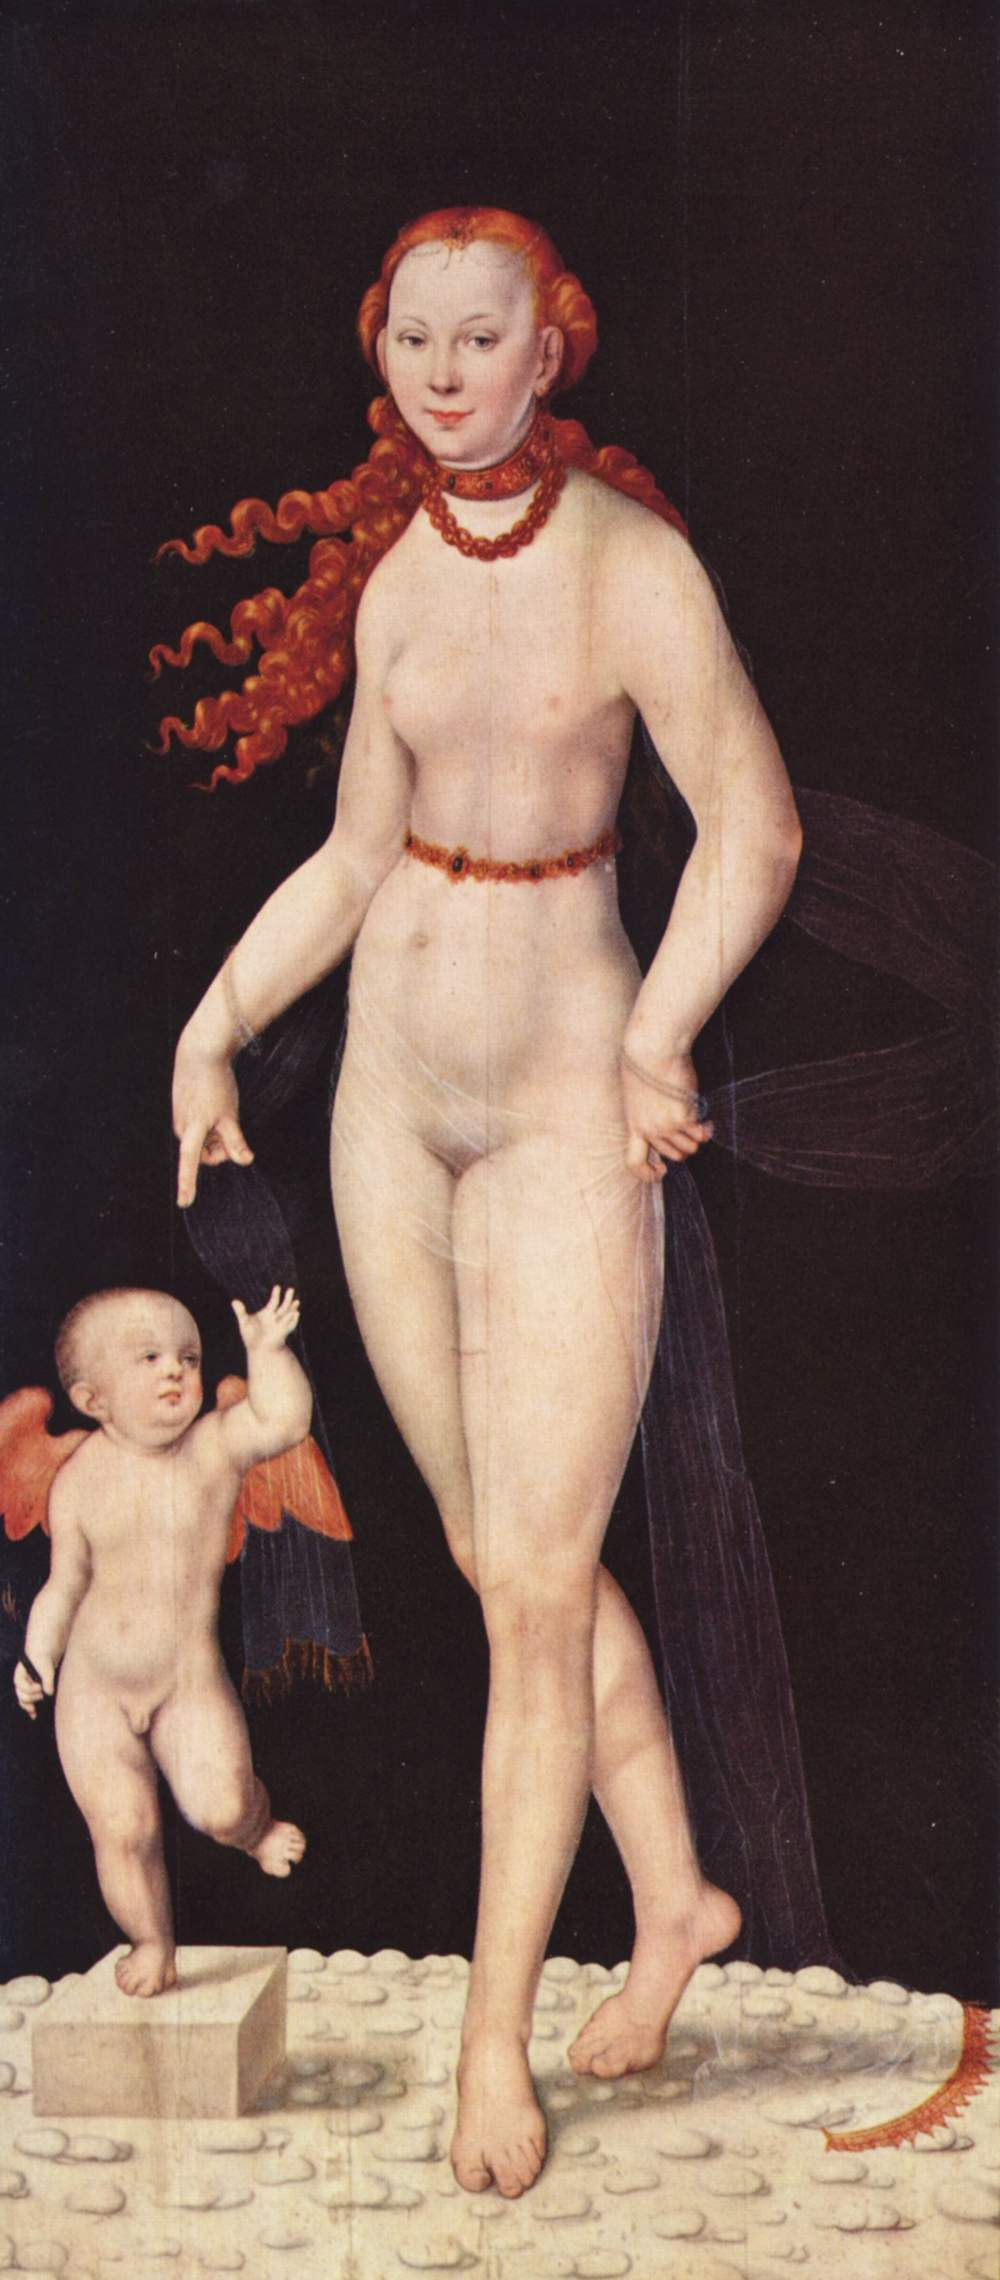
\includegraphics{6780765/Cupido.jpg}

}

\caption{Baroque AI}

\end{figure}

Venus und Cupido, Heinrich Bollandt, between circa 1620 and circa 1630.
https://commons.wikimedia.org/wiki/File:Heinrich\_Bollandt\_-\_Venus\_und\_Cupido.jpg
This work is in the public domain.

Example publications:

\begin{itemize}
\item
  \href{https://nfdi4culture.github.io/experimental-books-workshop/}{Exhibition
  catalogue demo: toc Baroque /toc} from Experimental Books --
  Re-imagining Scholarly Publishing, COPIM. Workshop URL:
  https://experimentalbooks.pubpub.org/programme-overview
\item
  \href{https://simonxix.github.io/scholarled_catalogue/}{Publishers
  catalogue demo: ScholarLed} A catalogue of ScholarLed presses built on
  a Quarto / Jupyter Notebook model for computational publishing. The
  publication is automatically updated daily to reflect any new books
  added by the publishers.
\item
  \href{https://nfdi4culture.github.io/cp4c/}{Proof of concept \#1} -
  Computational Publication: Computational Publishing for Collections -
  ADA CP Prototype \#1 - Nov 22
\item
  \href{https://nfdi4culture.github.io/art_catalogue_test/}{Proof of
  concept \#2} - To be confirmed, completion for end of April 2023. This
  contains all parts fully rendered: Cover, colophon, essay, collection,
  graph, TIB AV Portal, Semantic Kompakkt
\item
  semanticClimate: To be confirmed - customised research papers readers
  made for regional climate change action plans based on IPCC reports
  and sourcing content from open research repositories.
\item
  FSCI Summer School - publishing from collections class: To be
  confirmed, July 2023
\end{itemize}

This work is licensed under a Creative Commons Attribution-ShareAlike
4.0 International License.

\bookmarksetup{startatroot}

\hypertarget{colophon}{%
\chapter{Colophon}\label{colophon}}

\begin{itemize}
\tightlist
\item
  Fork title: Janacnl / catalogue-003
\item
  Author: Cornelius, Jana Lisa
\item
  ORCID: https://orcid.org/0009-0004-3404-2441
\item
  Date: 21.04.2023
\item
  DOI: 10.5281/zenodo.7852387
\item
  Repository URL: https://github.com/Janacnl/catalogue-003
\end{itemize}

PUBLISHING FROM COLLECTIONS USES OF COMPUTATIONAL PUBLISHIGN AND
LINKEDOPEN DATA

Open Science Lab - TIB Hannnover

First published 2023-03-30

Copyright © The Authors 2023 Licensed as
https://creativecommons.org/licenses/by-sa/4.0/

DOI: https://doi.org/10.5281/zenodo.7701161

\bookmarksetup{startatroot}

\hypertarget{catalogue-experiment-baroque-ai}{%
\chapter{Catalogue Experiment: Baroque
AI}\label{catalogue-experiment-baroque-ai}}

\begin{verbatim}
Nextcloud Markdown document link: https://tib.eu/cloud/s/qBx8SbqiPBBedye 
\end{verbatim}

\hypertarget{part-of-the-series-baroque-toc-1}{%
\section{Part of the series: Baroque
TOC}\label{part-of-the-series-baroque-toc-1}}

\begin{itemize}
\tightlist
\item
  Class instructions and all links:
  \url{https://nfdi4culture.github.io/class-ADA-CP-pipeline/}
\item
  Demo publication: \url{https://nfdi4culture.github.io/catalogue-003/}
\item
  Repo link: \url{https://github.com/NFDI4Culture/catalogue-003}
\end{itemize}

\begin{center}\rule{0.5\linewidth}{0.5pt}\end{center}

\hypertarget{add-your-name}{%
\section{Add your name:}\label{add-your-name}}

\begin{itemize}
\tightlist
\item
  Jana Cornelius
\end{itemize}

\hypertarget{text-editing}{%
\section{Text editing}\label{text-editing}}

\textbf{Bavaria} is a state in the south of Germany that is known for
its rich culture, history, and art. The state has a number of museums
and galleries that showcase the unique cultural heritage of the region.

One of the most famous museums in Bavaria is the \textbf{Bavarian
National Museum}, located in Munich. The museum houses a collection of
art and artifacts from the \emph{Middle Ages to the 20th century, with a
focus on Bavarian and German culture.} The museum also has a collection
of traditional Bavarian clothing and folk art.

Another notable museum in Bavaria is the \textbf{Pinakothek der
Moderne}, also located in Munich. The museum is dedicated to
\emph{modern and contemporary art,} with a collection that includes
works by famous artists such as Pablo Picasso and Andy Warhol.

In Nuremberg, the \textbf{Germanisches Nationalmuseum} is the largest
museum of \emph{cultural history} in Germany. The museum has a
collection of over 1.3 million objects that tell the story of German
culture and history from prehistoric times to the present day.

ChatGPT (2023): Museums of Bavaria. Online unter
https://chat.openai.com/c/6c3124a7-b1ab-47d5-86da-86a4f8f5fd8e {[}Abruf
am 20.04.2023{]}

\url{https://openai.com/blog/chatgpt}

\url{https://www.perplexity.ai/}

\bookmarksetup{startatroot}

\hypertarget{activity-paintings-catalogue-in-jupyter-notebook}{%
\chapter{Activity: Paintings catalogue in Jupyter
Notebook}\label{activity-paintings-catalogue-in-jupyter-notebook}}

Objective: Make a selection of nine paintings for the exhibition
catalogue to be selected from Wikidata and rendered multi-format in
Quarto.

The below Python code uses SPARQLWrapper to retrieve data from Wikidata
based on a SPARQL query.

Wikidata link: \url{http://www.wikidata.org/entity/Q18689231}

Title: Maria Theresa, Archduchess of Habsburg

Year: 1730

Creator: Rosalba Carriera

Copyright: public domain

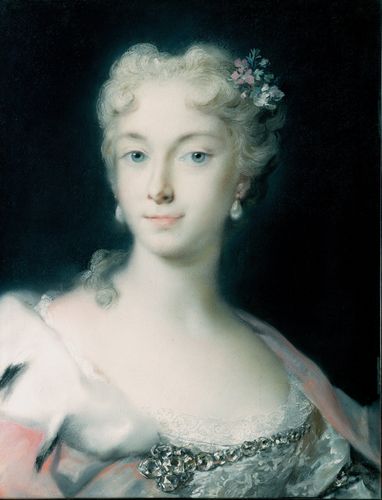
\includegraphics{paintings_files/figure-pdf/cell-2-output-2.png}

Wikidata link: \url{http://www.wikidata.org/entity/Q18689261}

Title: A Gentleman in a Gold Patterned Coat and Violet-Brown Cape

Year: 1727

Creator: Rosalba Carriera

Copyright: public domain

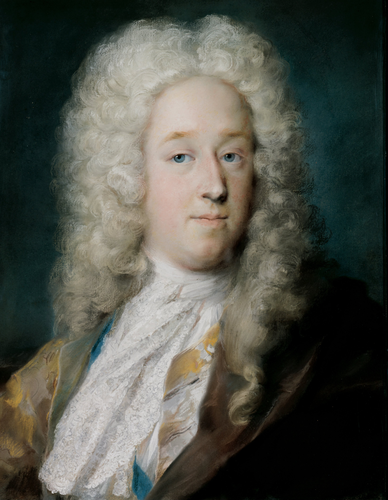
\includegraphics{paintings_files/figure-pdf/cell-2-output-4.png}

Wikidata link: \url{http://www.wikidata.org/entity/Q18689275}

Title: Louis XV of France as Dauphin

Year: 1720

Creator: Rosalba Carriera

Copyright: public domain

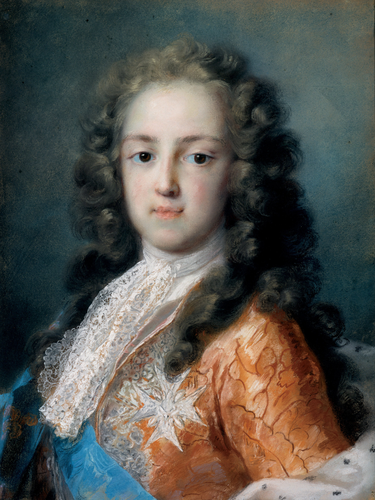
\includegraphics{paintings_files/figure-pdf/cell-2-output-6.png}

Wikidata link: \url{http://www.wikidata.org/entity/Q19266867}

Title: Las tres velas

Year: 1903

Creator: Joaquín Sorolla

Copyright: public domain

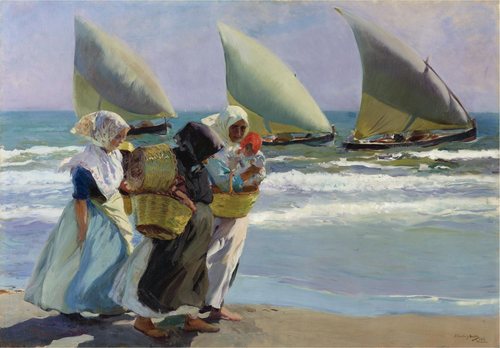
\includegraphics{paintings_files/figure-pdf/cell-2-output-8.png}

Wikidata link: \url{http://www.wikidata.org/entity/Q28798167}

Title: The Singer Faustina Bordoni (1697-1781) with a Musical Score

Year: 1724

Creator: Rosalba Carriera

Copyright: public domain

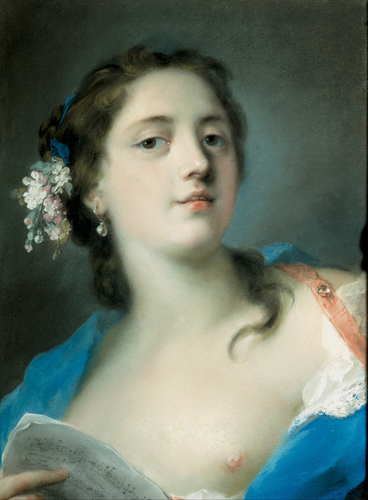
\includegraphics{paintings_files/figure-pdf/cell-2-output-10.png}

Wikidata link: \url{http://www.wikidata.org/entity/Q50326304}

Title: Judgement of Paris

Year: 1712

Creator: Adriaen van der Werff

Copyright: public domain

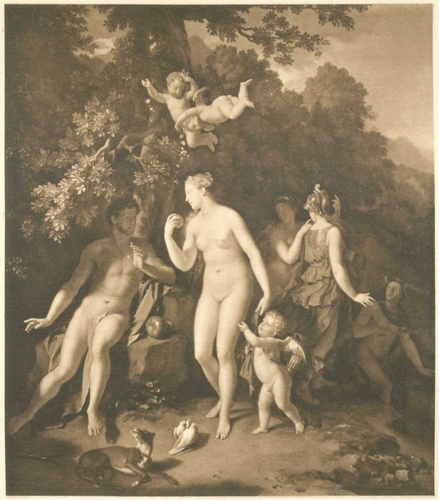
\includegraphics{paintings_files/figure-pdf/cell-2-output-12.png}

Wikidata link: \url{http://www.wikidata.org/entity/Q50326304}

Title: Judgement of Paris

Year: 1712

Creator: Adriaen van der Werff

Copyright: public domain

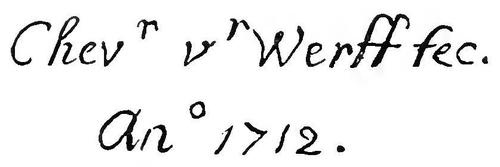
\includegraphics{paintings_files/figure-pdf/cell-2-output-14.png}

Wikidata link: \url{http://www.wikidata.org/entity/Q50327445}

Title: Youthful self-portrait

Year: 1765

Creator: Anton Graff

Copyright: public domain

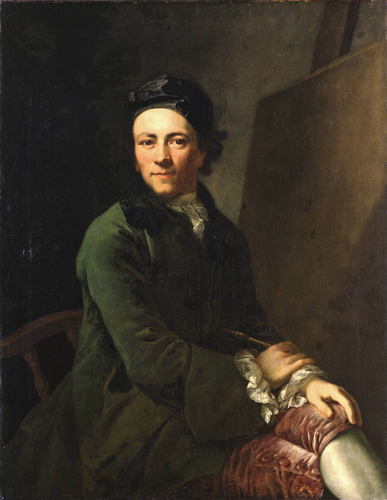
\includegraphics{paintings_files/figure-pdf/cell-2-output-16.png}

Wikidata link: \url{http://www.wikidata.org/entity/Q64541395}

Title: Portrait of Heinrich von Brühl

Year: 1753

Creator: Marcello Bacciarelli

Copyright: public domain

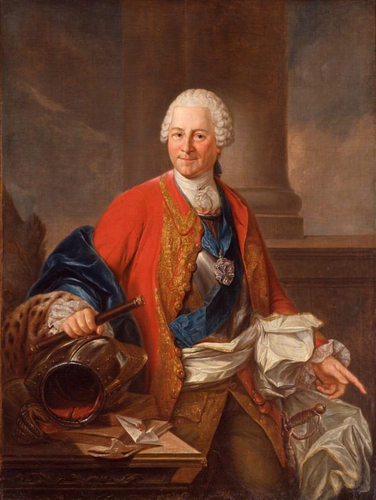
\includegraphics{paintings_files/figure-pdf/cell-2-output-18.png}

\bookmarksetup{startatroot}

\hypertarget{activity-embedded-video-in-jupyter-notebook}{%
\chapter{Activity: Embedded video in Jupyter
Notebook}\label{activity-embedded-video-in-jupyter-notebook}}

Objective: Running and editing Juypter Notebooks in MyBinder and
retrieving video and 3D models as embeds.

\hypertarget{video-embedding}{%
\section{Video embedding}\label{video-embedding}}

The below Python code experiments with retrieving video data via iframe
embedding.

\begin{verbatim}
<IPython.core.display.HTML object>
\end{verbatim}

\hypertarget{d-model-embedding}{%
\section{3D model embedding}\label{d-model-embedding}}

The below Python code experiments with retrieving 3D data via iframe
embedding.

\begin{verbatim}
<IPython.core.display.HTML object>
\end{verbatim}

\begin{verbatim}
<IPython.core.display.HTML object>
\end{verbatim}


\backmatter

\end{document}
